As with many modern software projects, this system was not built with a waterfall methodology. This means that a lot of testing was done in parallel with development and minor problems have been mitigated. The results presented here is the state of the project when development halted, when the project is a minimum viable product with the biggest issues fixed.

\subsection{Method of testing}
Finlands-svenska manssångarförbundet (FSM) has kindly provided recordings of each of the parts of a TTBB choir's rendition of Finlandia. The notes for these were not provided but sheet music of the same rendition was found online and manually verified to be correct. As a reminder, the system simply \textit{listens} to the input stream and then just notes what the current detected note in time is. A separate time-keeper was added, which samples the detected note at regular intervals. As long as the sample frequency is small enough, no information is lost. However, as was discussed, a performance of a piece is seldom an exact instance of the definition (sheet music), especially in terms of tempo. Certain sections may be dragged out, for example, for whatever reason. Dynamic time warping (DTW) was proposed as a solution to comparing the performance and the reference for its ability to focus on parallels between substructures rather than absolute similarity.

For Finlandia, sampling at 8th notes is sufficient, because it does not contain shorter notes than that. As the current goal is just to check that a detected note is correct, the system needs to know what note it should expect at that moment in time. This means that the sheet music can be transcribed to a sequence of 8th notes or represented as a time series where each data point is a MIDI number equally spaced in time. Quarter notes become two 8th notes, half notes become four 8th notes and so on. Figure \ref{fig:sheetEncoding} visualizes the time series using color for amplitude.

\begin{figure}[ht]
    \centering
    
\includegraphics[width=\textwidth]{./images/sheetEncoding.png}
    \caption{Sheet music of Finlandia as a time series, visualized with color for amplitude. To keep data points equally spaced in time, all notes are converted 8th notes. \label{fig:sheetEncoding}}
\end{figure}

Figure \ref{fig:sheetEncoding} is the same as the top part of Figure \ref{fig:performance-sheet}. The bottom part of that was a manually cleaned up version of the pitch detector's first effort, purely for demonstration purposes. DTW is only used to compare the recordings provided by FSM for a more proper test. In the real-time pitch detector, each note is directly tested as time goes on.

\subsection{Analysis of HPS iterations}
Each part of Finlandia was run through the system with 4, 5 and 6 for the number of HPS iterations. For these tests, the system is filtering out outliers and results of flat spectra. Figure \ref{fig:hpsTenor1} shows the comparison of one part. At a glance all versions are largely correct by looking at the substructures of the detected series and comparing them to the substructures of the reference. It's not obvious which time series did the best, but 6 iterations clearly did worst based on the amount of black in the diagram, which indicates a low note. Computing the error using DTW reveals that the error for 4 HPS iterations was 434, 352 for 5 iterations and 591 for 6 iterations. It can be hard to judge how good or bad a score of 352 is, but it clearly isn't optimal.

\begin{figure}[ht]
    \centering
    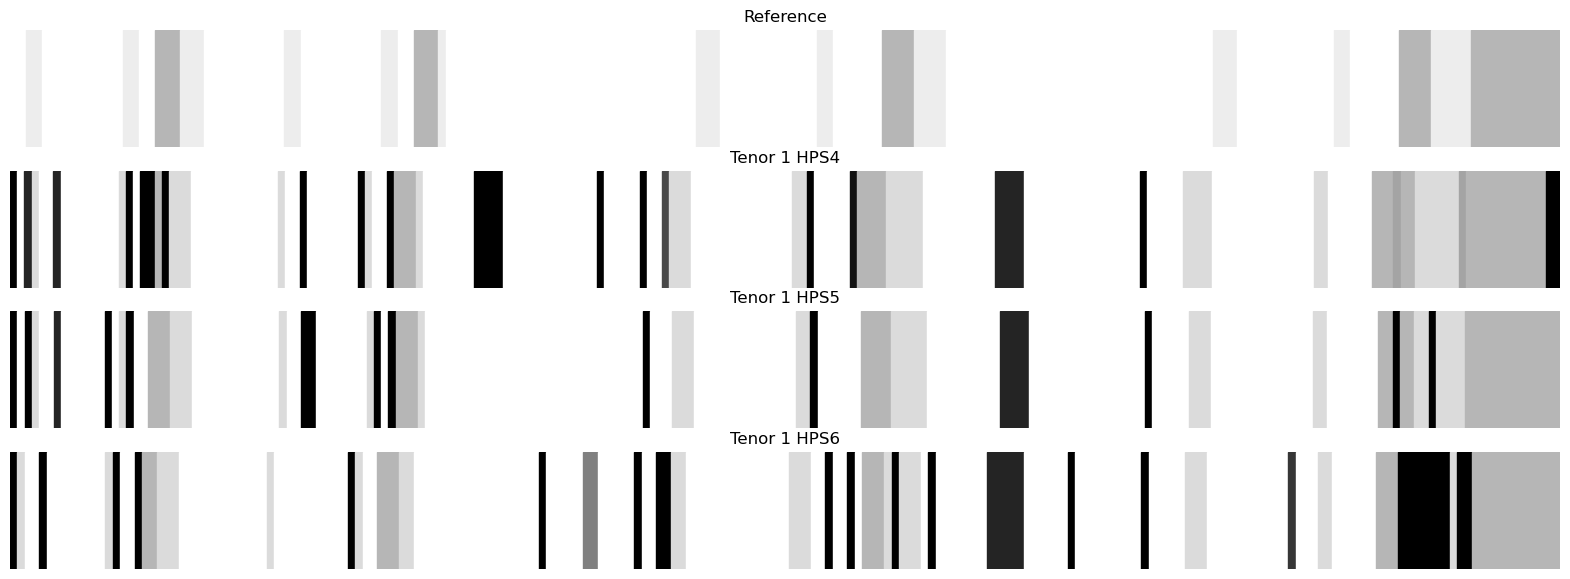
\includegraphics[width=\textwidth]{./images/hpsTenor1.png}
    \caption{Comparison of the First Tenor recordings with different number of HPS iterations. \label{fig:hpsTenor1}}
\end{figure}

The same analysis can be done for the rest of the parts shown in Figures \ref{fig:hpsTenor2}, \ref{fig:hpsBass1} and \ref{fig:hpsBass2}.

\begin{figure}[ht]
    \centering
    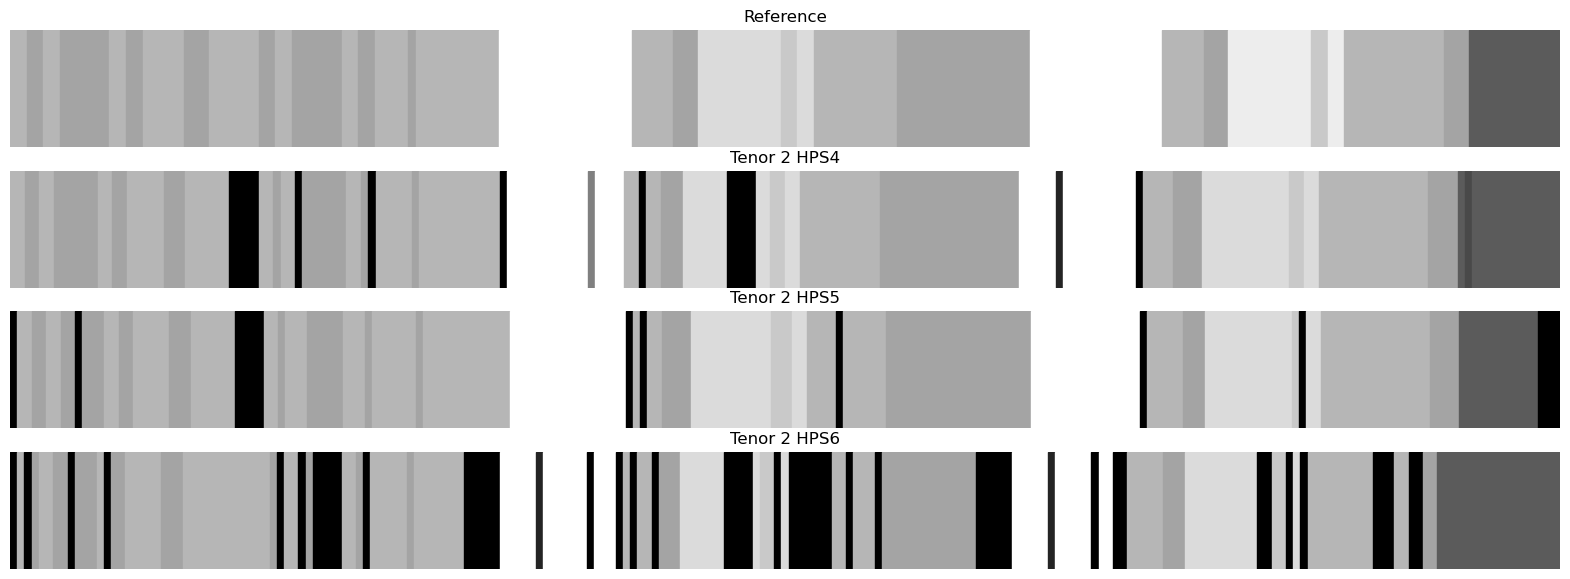
\includegraphics[width=\textwidth]{./images/hpsTenor2.png}
    \caption{Comparison of the Second Tenor recordings with different number of HPS iterations. \label{fig:hpsTenor2}}
\end{figure}


\begin{figure}[ht]
    \centering
    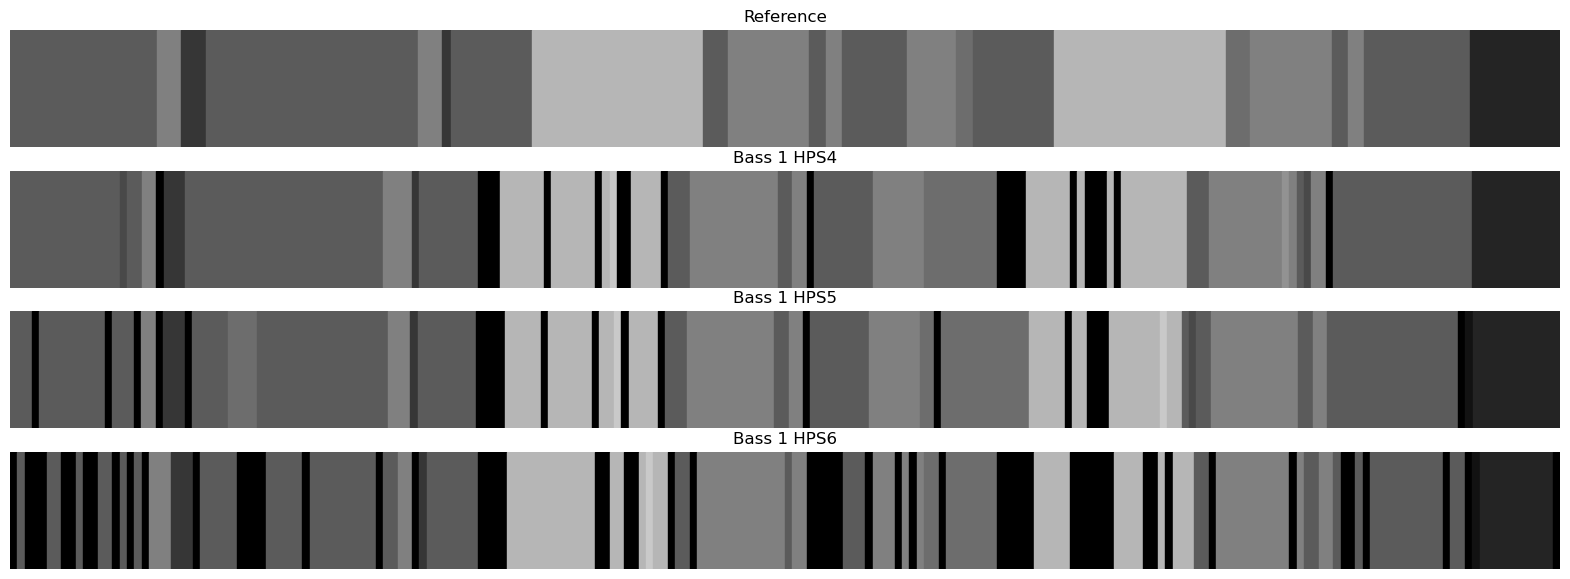
\includegraphics[width=\textwidth]{./images/hpsBass1.png}
    \caption{Comparison of the First Bass recordings with different number of HPS iterations. \label{fig:hpsBass1}}
\end{figure}


\begin{figure}[ht]
    \centering
    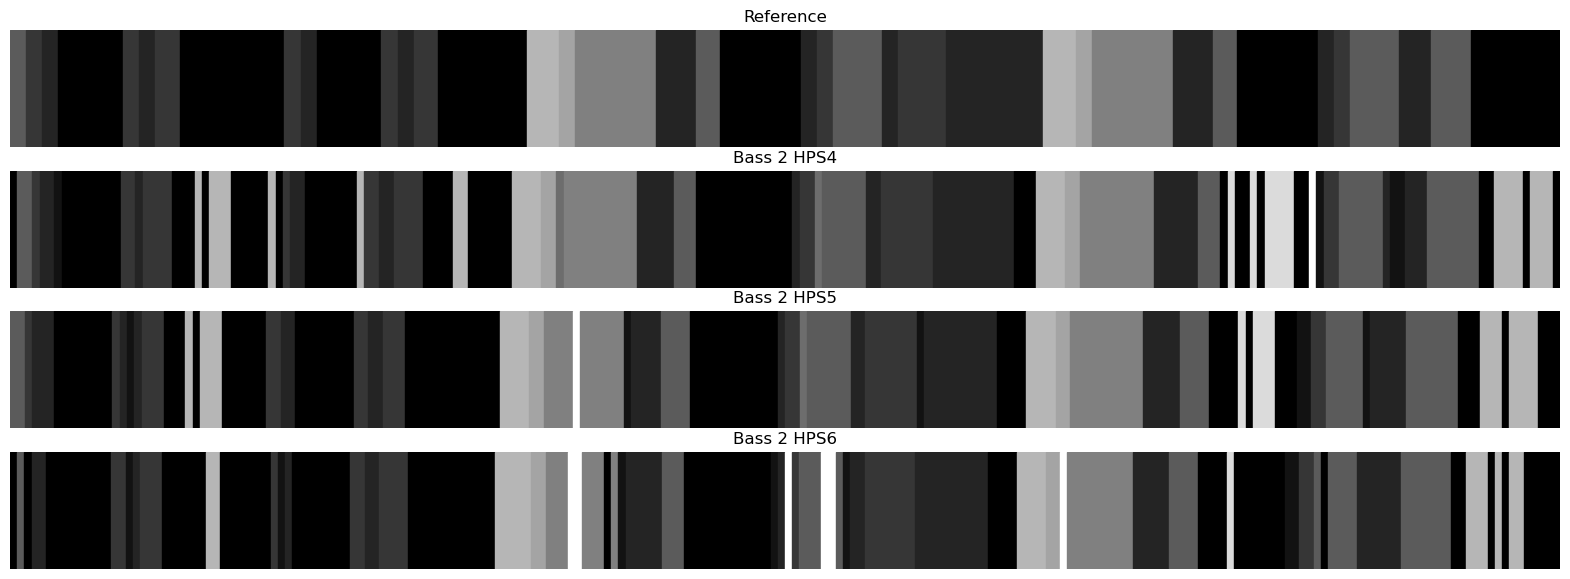
\includegraphics[width=\textwidth]{./images/hpsBass2.png}
    \caption{Comparison of the Second Bass recordings with different number of HPS iterations. \label{fig:hpsBass2}}
\end{figure}

Computing the average DTW error of the parts reveals that 5 iterations has the lowest error at 264.5. Again, hard to say how bad this score is, but the average for 6 iterations is 657.25 reveals at least that it's a big improvement. The average for 4 iterations is 299.75 which is still around 10\% worse than 5 iterations.

\subsubsection{Octave errors}
After outlier and flat spectra filtering, the most common type of error happens when HPS folds the spectrum in a way where multiple peaks remain. Assuming a monophonic singing, these remaining peaks are still harmonics. The system naively selects the greatest peak from these which results may result in note being in the wrong octave. For the tenors the system would go consistently lower and higher for the basses. The problem likely lies in the number of HPS iterations as based on the diagrams, it can be observed that 4 iteration HPS performs very well in certain parts and 6 iterations performs well in others. This strongly suggests that the best approach would be to have some sort of Dynamic HPS that can adjust the number of iterations depending on the number of peaks. One approach could be the do 4 iterations by default after which more are done depending on the number of remaining peaks. CFAR would be a strong candidate for this approach.

Figure \ref{fig:hpsOctaveErrors} is created by computing the remainder of the MIDI numbers modulo 12 to get octave indifferent notes. It clearly shows that most of the errors in the results regardless of HPS iterations are due to octave errors. In effect, it highlights the parts where the detector got the note wrong. This analysis is done to highlight the presence of octave errors and it does not imply that the system could automatically correct octave errors by comparing notes mod 12, as this could lead to false positives if the user sung an octave wrong, which is important.

\begin{figure}[ht]
    \centering
    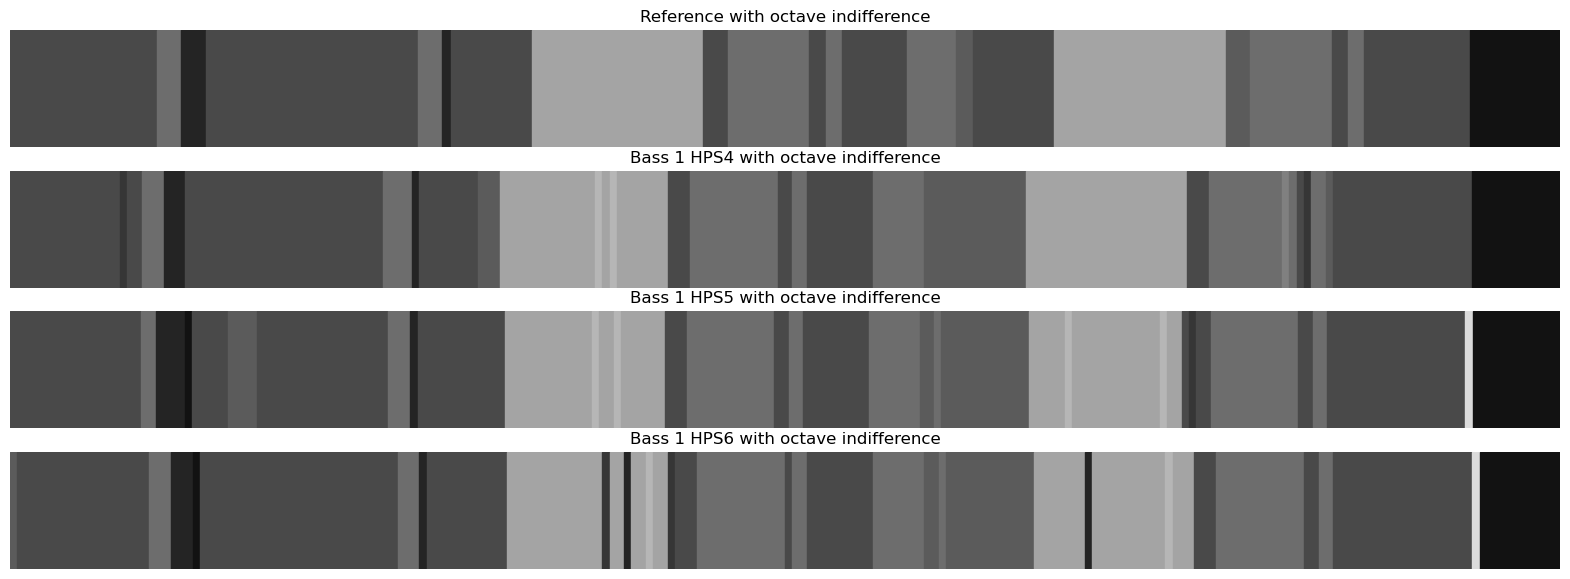
\includegraphics[width=\textwidth]{./images/hpsOctaveErrors.png}
    \caption{Comparison of HPS iterations with octave indifference. \label{fig:hpsOctaveErrors}}
\end{figure}


\subsection{Qualitative evaluation of responsivness}S
\subsection{Pitch detector accuracy}





\subsubsection{Piano}
\subsubsection{Voice}
\subsection{Pitch detector stability}
\subsection{Comparing FFT window sizes}
\subsection{Comparing peak pickers}
\subsection{Comparing FFT implementations}